\documentclass[tikz,border=0cm,dvipsnames,x11names,rgb]{standalone}

\usepackage{amsmath,amssymb,amsfonts}
\usetikzlibrary{calc,
fit,
shapes.misc,
shapes.geometric,
arrows.meta,
fadings,
matrix,
chains,
scopes,
positioning}

\usepackage{pgfplots}
\usepackage{pgfplotstable}
\pgfplotsset{compat=1.18}



\usepackage[]{fontspec}

\setmainfont{Latin Modern Roman}
\setmonofont{Latin Modern Math}
\renewcommand{\textsc}[1]{{\fontfamily{lmr}\selectfont \scshape #1}}

\usepackage[]{bm}

\makeatletter
\@ifundefined{fromRoot}{\newcommand{\fromRoot}[1]{../../#1}}{}

\def\input@path{{../..}{..}{.}{./svg}{./pgfplots}{./tikzpicture}}
%or: \def\input@path{{/path/to/folder/}{/path/to/other/folder/}}
\makeatother

\newcommand{\ra}[1]{\renewcommand{\arraystretch}{#1}}

\newcommand*{\gf}[1]{\acrshort{gf}($#1$)}%
\newcommand*{\mpn}[1]{\bm{P}_{#1}}%
\newcommand*{\pn}[1]{%
  \ifthenelse{\equal{#1}{}}{$\mpn{0}$}{$\mpn{#1}$}%
}%

\newcommand*{\pk}[3]{%
  \ifthenelse{\equal{#1}{#2}}{\textcolor{red}{\phantom{.}$p_0$\phantom{.}}}{\phantom{.}$p_#3$\phantom{.}}%
}%


\newcommand*{\placeholderreg}{\includegraphics[width=\linewidth, height=.25\textheight, keepaspectratio = true]{figures/certified_xilinx.png}}%
\newcommand*{\placeholder}[1]{\includegraphics[#1]{figures/certified_xilinx.png}}%

\newcommand*{\snr}{\acrshort{snr}}%
\newcommand*{\snrs}{\acrshortpl{snr}}%

\newcommand*{\mpd}[0]{p_\Delta}%
\newcommand*{\mpo}[0]{p_\omega}%
\newcommand*{\pd}[0]{$\mpd$}%
\newcommand*{\po}[0]{$\mpo$}%
\newcommand*{\mpfa}[0]{\mathcal{P}_{fa}}%
\newcommand*{\mpmd}[0]{\mathcal{P}_{md}}%
\newcommand*{\pfa}[0]{\acrshort{pfa}}%
\newcommand*{\pmd}[0]{\acrshort{pmd}}%
\newcommand*{\mnorm}[1]{\mathcal{L}_{#1}}%
\newcommand*{\norm}[1]{$\mnorm{#1}$}%
\newcommand*{\fft}{\acrshort{fft}}%
\newcommand*{\mfft}[1]{\mathcal{F}(#1)}%
\newcommand*{\mifft}[1]{\mathcal{F}^{-1}(#1)}%
\newcommand*{\ts}{\acrshort{ts}}%

\newcommand*{\cpp}[1]{C\textrm{++#1}}%
\newcommand*{\na}{\textrm{\textcolor{SlateGray4}{N/A}}}%

\newcommand*{\vect}[1]{\bm{#1}}%
\newcommand*{\mat}[1]{\bm{\mathrm{#1}}}%

\newcommand*{\task}[1]{\mathcal{T}_{#1}}%

\newcommand*{\sdr}{\acrshort{sdr}}%
\newcommand*{\fpga}{\acrshort{fpga}}%

\newcommand*{\rikiki}{\fontsize{4}{6}\selectfont}%



\begin{document}

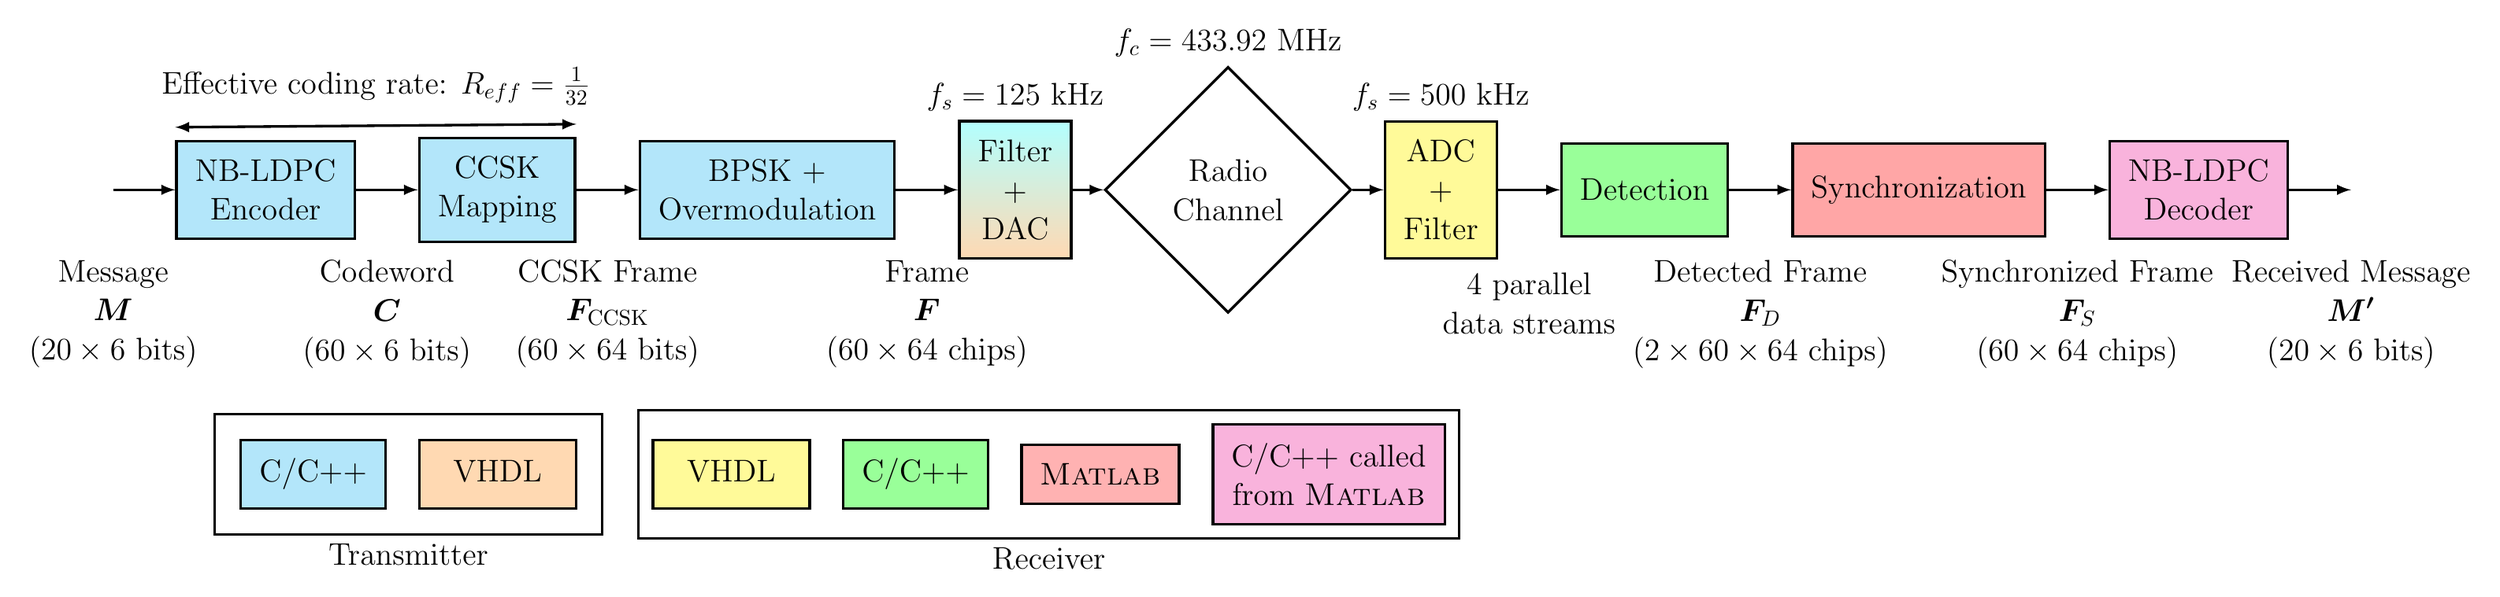
\begin{tikzpicture} [-latex,
    >=latex,
    auto,
    very thick,
    main node/.style={rectangle, fill = white!35, draw,
        align=center, inner sep = 3 mm},
    every node/.style={font=\Large}
  ]

  \node [main node,
    fill=cyan!30,
    align=center,
    minimum height = 1.5cm
  ] (nbenc) at (0, 0) {NB-LDPC\\Encoder};

  \draw ($(-1, 0) + (nbenc.west)$) -> (nbenc.west)
  node [pos=0, align=center, below = 1cm] (M) {Message\\
      $\vect{M}$\\($20 \times 6$ bits)};

  \node [main node,
    fill=cyan!30,
    minimum height = 1.5cm,
    %minimum width = 3cm,
    right = 1cm of nbenc
  ] (ccskm) {CCSK\\Mapping};

  \draw (nbenc.east) -> (ccskm.west)
  node [midway, align=center, below = 1cm] (cw) {Codeword\\
      $\vect{C}$\\($60 \times 6$ bits)};

  \node [main node,
    fill=cyan!30,
    minimum height = 1.5cm,
    %minimum width = 3cm,
    right = 1cm of ccskm
  ] (bpskm) {BPSK $+$\\Overmodulation};

  \draw (ccskm.east) -> (bpskm.west)
  node [midway, align=center, below = 1cm] (M) {CCSK Frame\\
      $\vect{F}_{\mathrm{CCSK}}$\\($60 \times 64$ bits)};

  \node [main node,
  top color = cyan!30,
  bottom color = orange!30,
  align=center,
  minimum height = .75cm,
  minimum width = .5cm,
  label = above:{$f_s = 125$ kHz},
  right = 1 cm of bpskm
  ] (dac) {Filter\\$+$\\DAC};

  \node [diamond,
  fill = white!35,
  draw,
  align=center,
  %minimum height = 1.5cm,
  %minimum width = 2cm,
  fill = white,
  inner sep = 3 mm,
  label=above:{$f_c = 433.92$ MHz},
  right = .5 cm of dac
  ] (chan) {Radio\\Channel};

  \node [main node,
  align=center,
  minimum height = .75cm,
  minimum width = .5cm,
  fill = yellow!40,
  label = above:{$f_s = 500$ kHz},
  right = .5cm of chan
  ] (adc) {ADC\\$+$\\Filter};

  \draw (bpskm.east) -- (dac.west)
  node [midway, align=center, below = 1cm] (M) {Frame\\
  $\vect{F}$\\($60 \times 64$ chips)};

  \draw (dac.east) -- (chan.west);
  \draw (chan.east) -- (adc.west);

  \node [main node,
    minimum height = 1.5cm,
    fill = green!40,
    %minimum width = 3cm,
    right = 1 cm of adc
  ] (ccskd)  {Detection};


  \draw (adc.east) -- (ccskd.west)
  node [midway, align=center, below = 1.2cm] (M) {$4$ parallel\\data streams};

  \node [main node,
    fill = red!35,
    minimum height = 1.5cm,
    %minimum width = 3cm,
    right = 1 cm of ccskd
  ] (ccsks) {Synchronization};

  \draw (ccskd.east) -> (ccsks.west)
  node [midway, align=center, below = 1cm] (M) {Detected Frame\\$\vect{F}_D$\\
      ($2 \times 60 \times 64$ chips)};

  \node [main node,
    fill = magenta!30,
    minimum height = 1.5cm,
    right = 1cm of ccsks
  ] (nbdec) {NB-LDPC\\Decoder};



  \draw (ccsks.east) -> (nbdec.west)
  node [midway, align=center, below = 1cm] (M) {Synchronized Frame\\$\vect{F}_S$\\
      ($60 \times 64$ chips)};


  \draw (nbdec.east) -> ($(1, 0) + (nbdec.east)$)
  node [pos=1, align=center, below = 1cm] (M) {Received Message\\
      $\vect{M'}$\\
      ($20 \times 6$ bits)};

  \draw [latex-latex] ($(0, .2) + (nbenc.north west)$) -- ($(0, .2) +
  (ccskm.north east)$)
  node [midway, align=center, above = .2cm] (Mp) {Effective coding rate:
      $R_{eff} = \frac{1}{32}$};




  %\draw ($(-1, 0) + (ccskd_z.west)$) -> (ccskd_z.west);

  %\draw (ccsks.east) -> ($(1, 0) + (ccsks.east)$);

  %\draw [dashed, color = red!50!gray, -] (anchor.south west) -- (frame_chosen.north west);
  %\draw [dashed, color = red!50!gray, -] (anchor.south east) -- (frame_chosen.north east);

  \node [
    main node,
    draw,
    anchor = north east,
    fill=cyan!30,
  ] at ($(cw.south) - (0, 1)$) (emcc) {C/\cpp{}};
  \node [
    main node,
    draw,
    right = .5cm of emcc,
    fill=orange!30,
  ] (emvl) {\phantom{/}VHDL\phantom{/}};

  \node[
    draw,
    inner sep = 4 mm,
    fit = (emcc) (emvl)
  ] (emfit) {};
  \node [anchor = north, inner sep = 1 mm] at (emfit.south) {Transmitter};

  \node [
    main node,
    draw,
    right = 1.2 cm of emvl,
    fill=yellow!40,
  ] (rcvl) {\phantom{/}VHDL\phantom{/}};
  \node [
    main node,
    draw,
    right = .5cm of rcvl,
    fill=green!40,
  ] (rccc) {C/\cpp{}};
  \node [
    main node,
    draw,
    right = .5cm of rccc,
    fill=red!30,
  ] (rcm) {\textsc{Matlab}};
  \node [
    draw,
    main node,
    align = center,
    right = .5cm of rcm,
    fill=magenta!30,
  ] (rcmc) {C/\cpp{} called\\from \textsc{Matlab}};

  \node[
    draw,
    inner sep = 2.1 mm,
    fit = (rcvl) (rcmc)
  ] (rcfit) {};
  \node [anchor = north, inner sep = 1 mm] at (rcfit.south) {Receiver};

\end{tikzpicture}

\end{document}
